\documentclass[10pt,aspectratio=169]{beamer}

% All the boilerplate is in deslides.sty
\usepackage{deslides}

\author{Ji\v{r}\'i Lebl}

\institute[OSU]{%
Oklahoma State University%
%Departemento pri Matematiko de Oklahoma {\^S}tata Universitato%
}

\title{9. Autonomous equations\\(Notes on Diffy Qs, 1.6)}

\date{}

\begin{document}

\begin{frame}
\titlepage

%\bigskip

\begin{center}
The textbook: \url{https://www.jirka.org/diffyqs/}
\end{center}
\end{frame}

\begin{frame}
$\dfrac{dx}{dt} = f(x)$\quad
(equation independent of time)
is called an
\emph{autonomous equation}.

\medskip
\pause

\hspace*{3.1in} 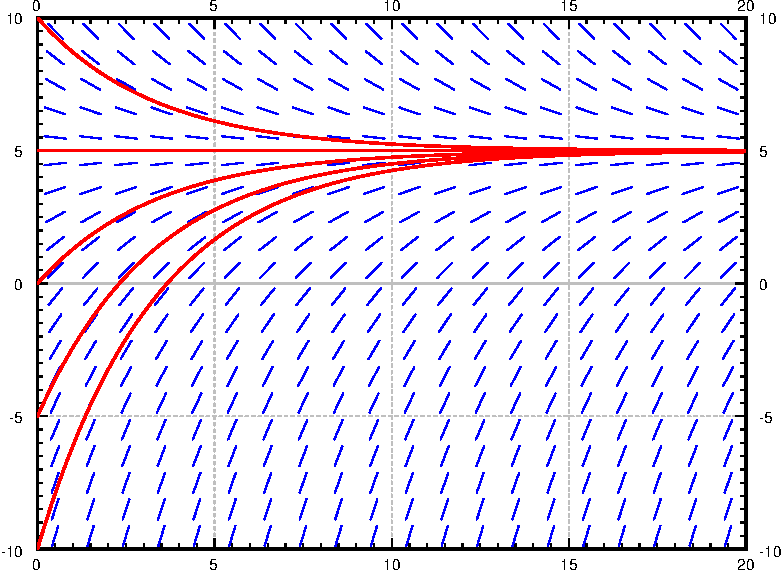
\includegraphics[width=2.2in]{../figures/2-2-coffee}

\hspace*{3.1in} $x' = 0.3(5-x)$\quad (i.e., $k=0.3$, $A=5$)

\vspace*{-1.8in}

\textbf{Example:} The cooling coffee problem

\medskip

$\dfrac{dx}{dt} = k (A-x)$
\quad
(Newton's law of cooling)

\medskip

$x$=temperature of coffee, $t$=time,

$A$=ambient temperature, $k$=constant

\medskip
\pause

The solution $x=A$ is called

an \emph{equilibrium solution}.

\medskip
\pause

Equilibrium solutions happen when $f(x)=0$.

\medskip
\pause

Call an $x$ such that $f(x)=0$ a \emph{critical point}

($f(5)=0$ in the plot)

\medskip
\pause

The critical point $x=A=5$ is \emph{stable},

small changes in initial condition still lead to the solution approaching
$x=5$ as $t \to \infty$.

\medskip
\pause

A critical point that is not stable is called \emph{unstable}.

\end{frame}

\begin{frame}
%\diffyincludegraphics{width=3in}{width=4.5in}{2-2-logistic}

% \caption{The slope field and some solutions of
% $x' = 0.1\,x\,(5-x)$.\label{2.2:logisticfig}}
%}
Consider the \emph{logistic equation}:
~
$x'= kx(M-x)$,~
for some $k > 0$ and $M > 0$.

\medskip
\pause

Common model for population where there is a maximum sustainable population $M$.

(less catastrophic than $x'=kx$)

\medskip
\pause

\textbf{Example:} $x' = 0.1 x(5-x)$

\vspace*{-\baselineskip}

\hspace*{3.1in} 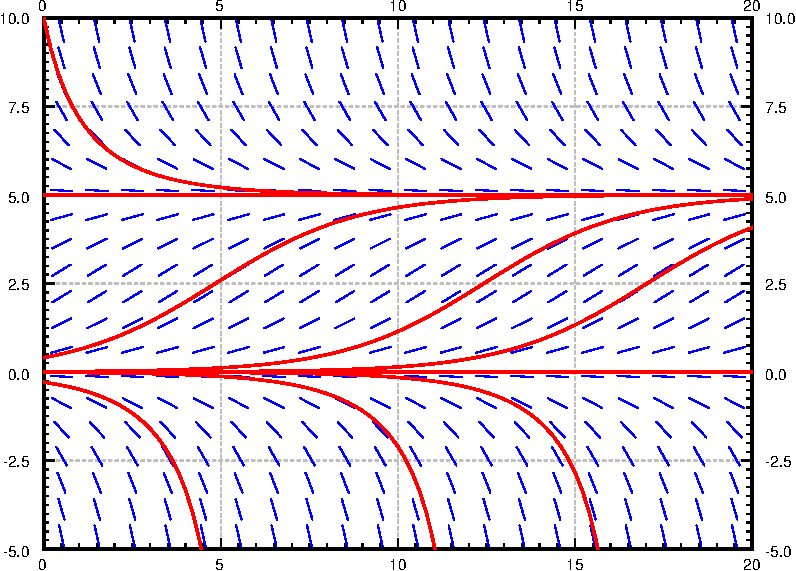
\includegraphics[width=2.2in]{../figures/2-2-logistic}

\vspace*{-1.4in}
\pause

Two critical points $x=0$ and $x=5$.

\pause
$x=0$ is unstable, \pause $x=5$ is stable.

\medskip
\pause

By inspection,

\medskip

$\displaystyle
\lim_{t\to \infty} x(t) = 
\begin{cases}
5 & \text{if } \; x(0) > 0 , \\
0 & \text{if } \; x(0) = 0 , \\
\text{DNE ~~or~~ } {-\infty} & \text{if } \; x(0) < 0 . \\
\end{cases}
$

\medskip
\pause

\textbf{Note:} Picture not enough to decide for $x(0) < 0$.
\pause
~
$x(t)$ may not exist for all time $t$.

\medskip
\pause

So to find long term behavior, $x(t)$ for very large $t$, we don't need to solve.

\end{frame}

\begin{frame}
To find $\lim\limits_{t \to \infty} x(t)$, enough to look at a \emph{phase diagram} (or \emph{phase portrait}):

\pause
1) Draw the $x$ axis (vertical).

\pause
2) Mark the critical points.

\pause
3) Draw an up arrow between where $f(x) > 0$ and down arrow where $f(x) <
0$.

\medskip
\pause

E.g.: $x' = f(x) = 0.1x(5-x)$

\bigskip
\pause

\quad\subimport*{../figures/}{2-2-l-phasedia.pdf_t}

\pause
\vspace*{-1.49in}

\hspace*{1in} 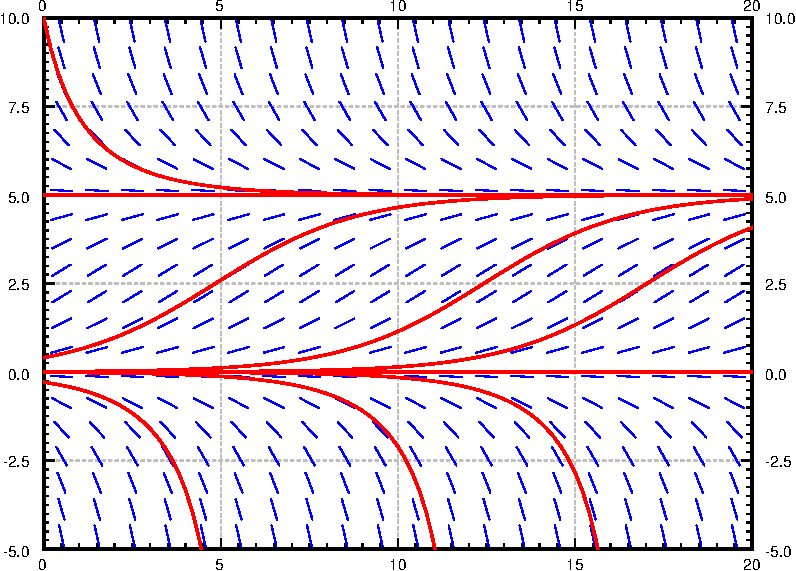
\includegraphics[width=2.2in]{../figures/2-2-logistic}

\medskip
\pause

Enough to note that $x=0$ and $x=5$ solve $0.1x(5-x)=0$.

\pause
Graph $f(x) = 0.1x(5-x)$,
\pause
or plug in a few points,

\pause
e.g.,
$f(6) = -0.6 < 0$,
\pause 
~$f(1) = 0.4 > 0$,
\pause
~$f(-1) = -0.6 < 0$

\pause
\vspace*{-1.8in}
\hspace*{3.35in}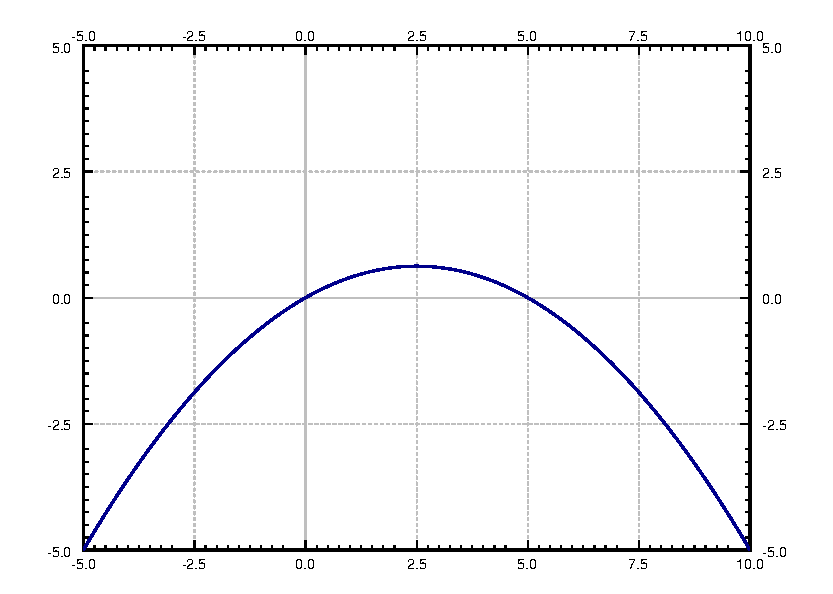
\includegraphics[width=2.3in]{figures/01x5mx}

\hspace*{3.5in} {\small Graph of $y=f(x)=0.1x(5-x)$}

\end{frame}

\begin{frame}
Armed with a phase diagram, easy to sketch solutions.

\vspace*{3.2in}

\end{frame}

\begin{frame}
Classifying critical points is also easy:

\medskip

\quad\subimport*{../figures/}{2-2-ph-class.pdf_t}

\medskip
\pause

\textbf{Remark:} If one arrow points in and one out, sometimes called
\emph{semistable}.

\medskip
\pause

Unstable points tend to be bad news:

\pause
Small changes in initial conditions lead to different outcomes.

\end{frame}

\begin{frame}
\textbf{Example:}
Consider the logistic equation with harvesting.

\pause
An alien race really likes to eat humans,

\pause
they harvest $h$ million humans per year.

\pause

$x$=millions of humans on the planet,
\pause
$t$=time in years,

\pause
$M$=limiting population when no harvesting.

\pause
$k > 0$ is a number depending on how quickly humans multiply.

\medskip
\pause

Equation becomes: ~
$x' = kx(M-x) - h$.

\medskip
\pause

Find critical points ~(solve~
$kx(M-x) - h = -kx^2+kMx - h  = 0$)

\medskip
\pause

There are two (quadratic formula).  Give them names:

$A = \dfrac{kM + \sqrt{{(kM)}^2 - 4hk}}{2k}$, \qquad
$B = \dfrac{kM - \sqrt{{(kM)}^2 - 4hk}}{2k}$.

\pause
\medskip

$3$ possibilities:
$A > B$, or $A=B$, or $A$ and $B$ both complex
(i.e.\ no real solutions).

\end{frame}

\begin{frame}
For example, let $M=8$ and $k=0.1$.

\medskip
\pause

Harvest $h=1$ million:

\vspace*{-\baselineskip}

 \hspace*{1.5in} 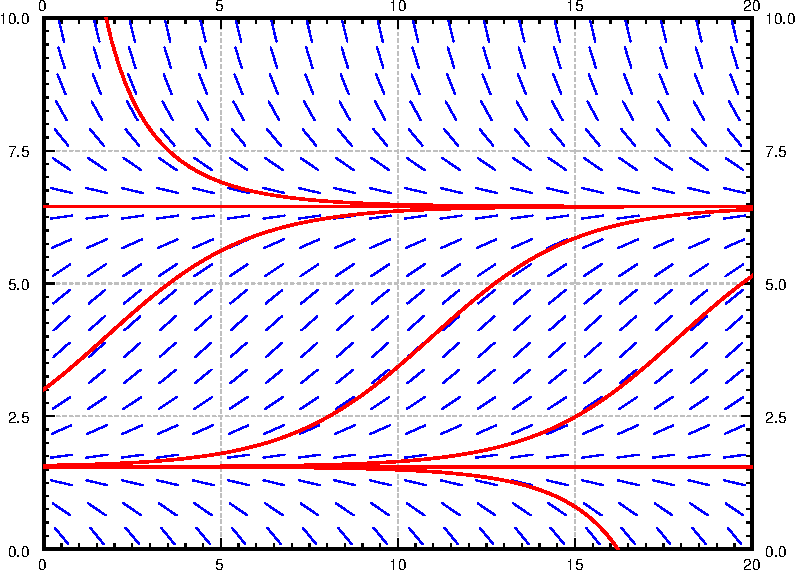
\includegraphics[width=3in]{../figures/2-2-logistic-h1}

 \hspace*{1.5in} $x' = 0.1\,x\,(8-x)-1$

\pause
\medskip

$A \approx 6.45$, \pause stable
\pause
\qquad
$B \approx 1.55$, \pause unstable

\medskip
\pause

As long as there are at least 1.55 million humans,
the harvesting is sustainable.

\medskip
\pause

If there is an earthquake and population drops below $B$,

\pause
the alien race becomes vegetarian. (not good for us either)
\end{frame}

\begin{frame}
Now harvest $h=1.6$:

\vspace*{-\baselineskip}

\hspace*{1.5in} 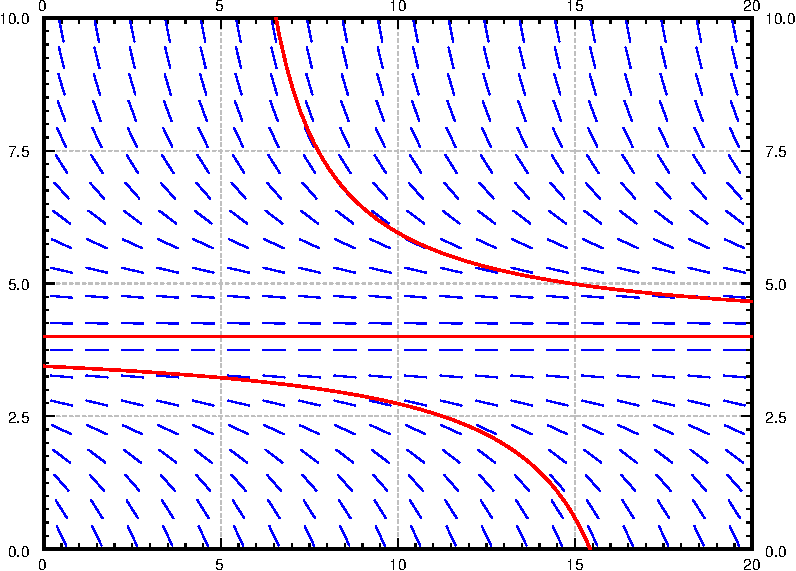
\includegraphics[width=3in]{../figures/2-2-logistic-hc}

\hspace*{1.5in} $x' = 0.1\,x\,(8-x)-1.6$.

\medskip
\pause

$A=B=4$, only one (unstable) critical point.

\medskip
\pause

If population starts above $4$ million, it will tend towards $4$ million.

\medskip
\pause

If the population drops below $4$ million, humans die out.

\end{frame}

\begin{frame}
Now harvest $h=2$ million per year.

\medskip
\pause

\qquad 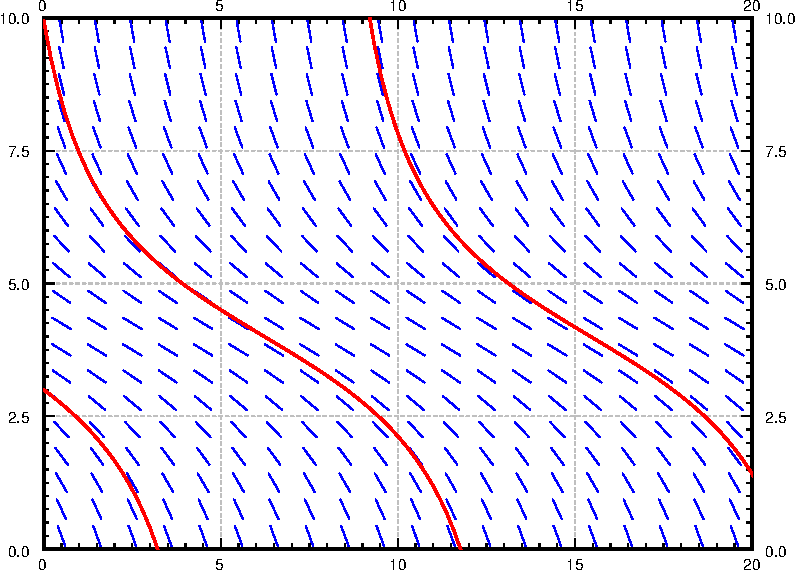
\includegraphics[width=3in]{../figures/2-2-logistic-h2}

\qquad $x' = 0.1\,x\,(8-x)-2$.

\medskip
\pause

No critical points.
\pause
Population always goes to 0.

\end{frame}

\end{document}
